\subsection{Quantitative Evaluation}
\label{subsec:quantitative-eval}

Here we address requirements R2 and R3. First, we compute project profiles. These profiles show the distribution of work-related dependencies in a project. Second, we evaluate whether the work on files can be predicted.

Before assessing project profiles, we make the following consideration. Our metrics define four classes:
\begin{inparaenum}[\itshape i)]
	\item low distance low co-evolution;
	\item high distance low co-evolution;
	\item low distance high co-evolution;
	\item high distance high co-evolution.
\end{inparaenum} \Cref{fig:pairs-on-space} helps clarifying these four classes. In fact, except for values of distance equal to 0, it is possible to see how the density of file pairs is higher when the distance is low. This is a normal situation in project where highly related files are stored closely to each other in the file system. Conversely, the dots on the top right of the plot mark files which are very distant to each other but still highly correlated. These can be, for instance, logical dependencies that can happen because of bad modularization of the project.

Hidden work dependencies belong to the last mentioned case, i.e. files are distant in the file tree but they have similar time series. According to this consideration we computed the project profiles in \Cref{fig:project-analysis}. We observe three types of processes. First, several projects have hardly any hidden work dependencies. Second, several have a moderate degree between 10\% and 20\%. Third, the project \textit{Biglist} has a high share of hidden dependencies. This hints at the possibility for better organizing the project according to good modularization best practices. That means, the project can be restructured in a way to reduce the unwanted side-effect the work on one file produces on other files.
%% Please add the following required packages to your document preamble:
% \usepackage{multirow}
%\setlength{\textfloatsep}{0.1cm}
\begin{table}[h]
\centering
%\caption{Project assessment schema}
\label{tab:project-assessment-schema}
\begin{tabular}{cccc}
\multirow{4}{*}{\rot{Distance $d$}} & \multicolumn{3}{c}{Degree of co-evolution $\chi$}                                 \\
&                           & \textit{low}        & \textit{high}                                      \\ \cline{3-4} 
& \multicolumn{1}{c|}{\textit{low}}  & irrelevant & \multicolumn{1}{c|}{orderly}              \\
& \multicolumn{1}{c|}{\textit{high}} & orderly    & \multicolumn{1}{c|}{\textbf{interesting}} \\ \cline{3-4} 
\end{tabular}
\end{table}

%\rot{Distance $d$}


%\begin{figure}
%\centering
%
\includegraphics[width=0.3\linewidth]{figures/assessment-diagram}
%\caption{Project assessment diagram}
%\label{fig:assessment-diagram}
%\end{figure}
\begin{figure}[t]
	\begin{subfigure}[b]{.51\textwidth}
		\centering
		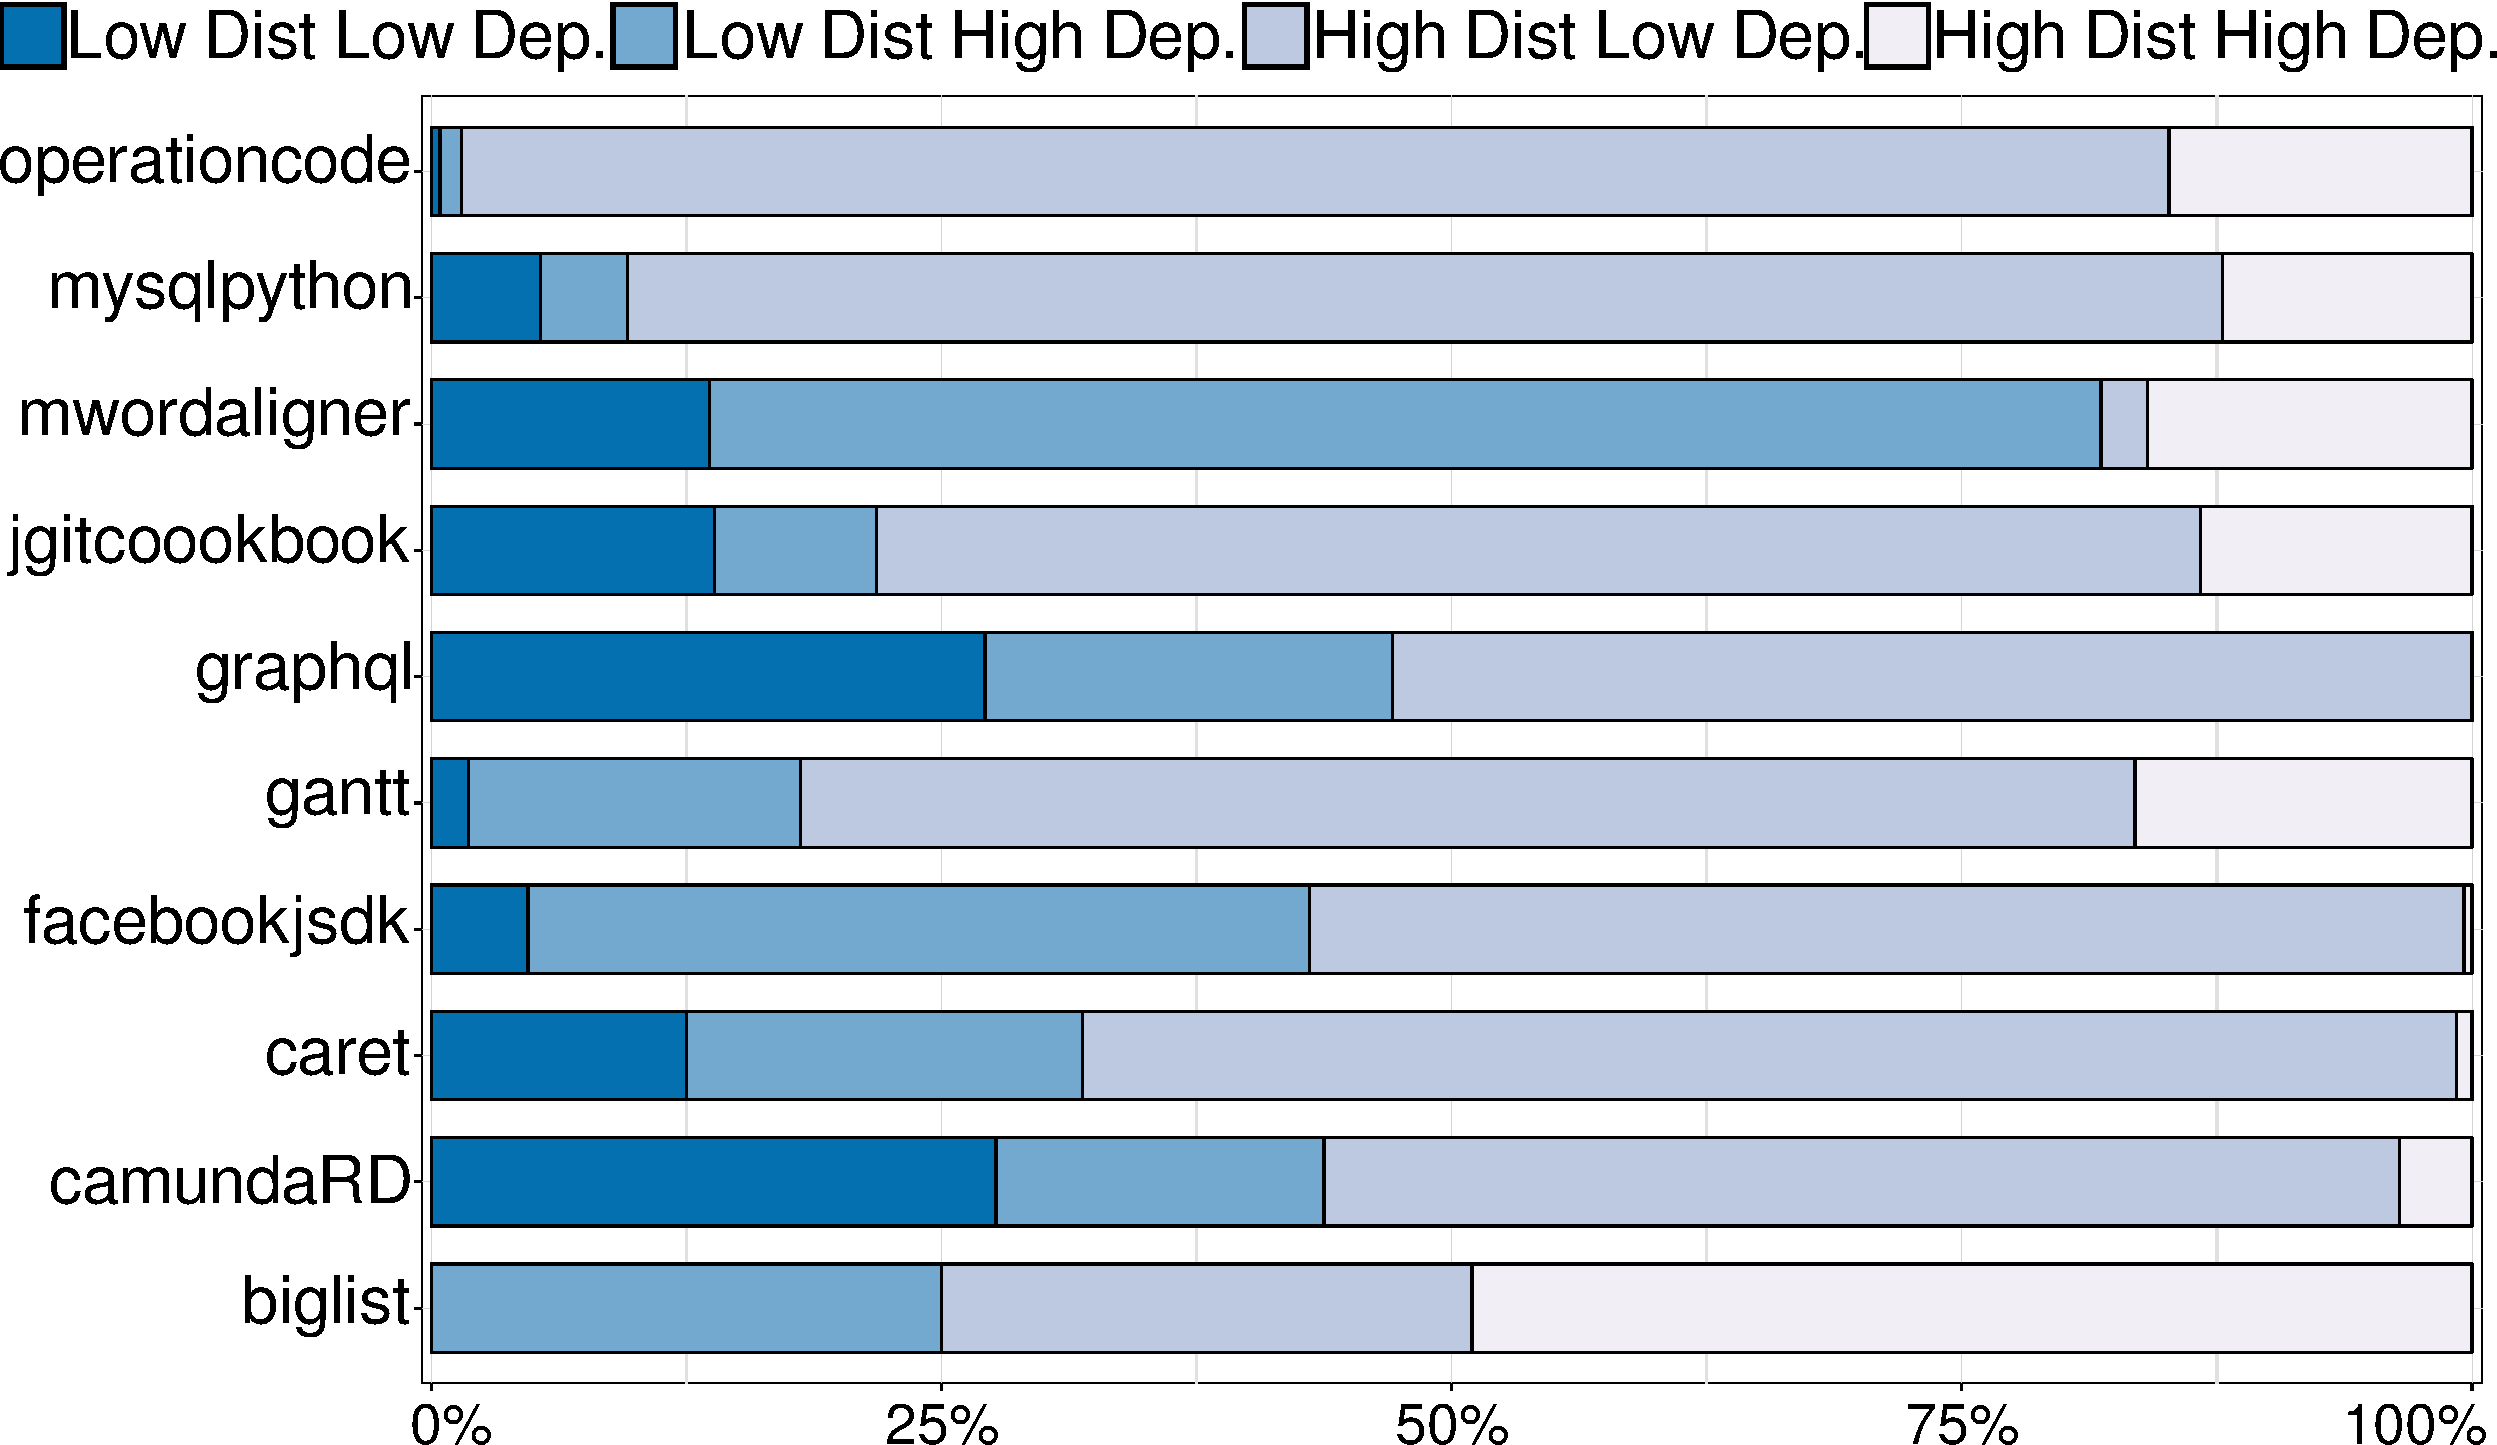
\includegraphics[width=.98\linewidth]{bpm2017/figures/Project-Analysis-Barchart-crop.pdf}
		\caption{Evaluation on real projects}
		\label{fig:project-analysis}
	\end{subfigure}~
	\begin{subfigure}[b]{.47\textwidth}
		\centering
		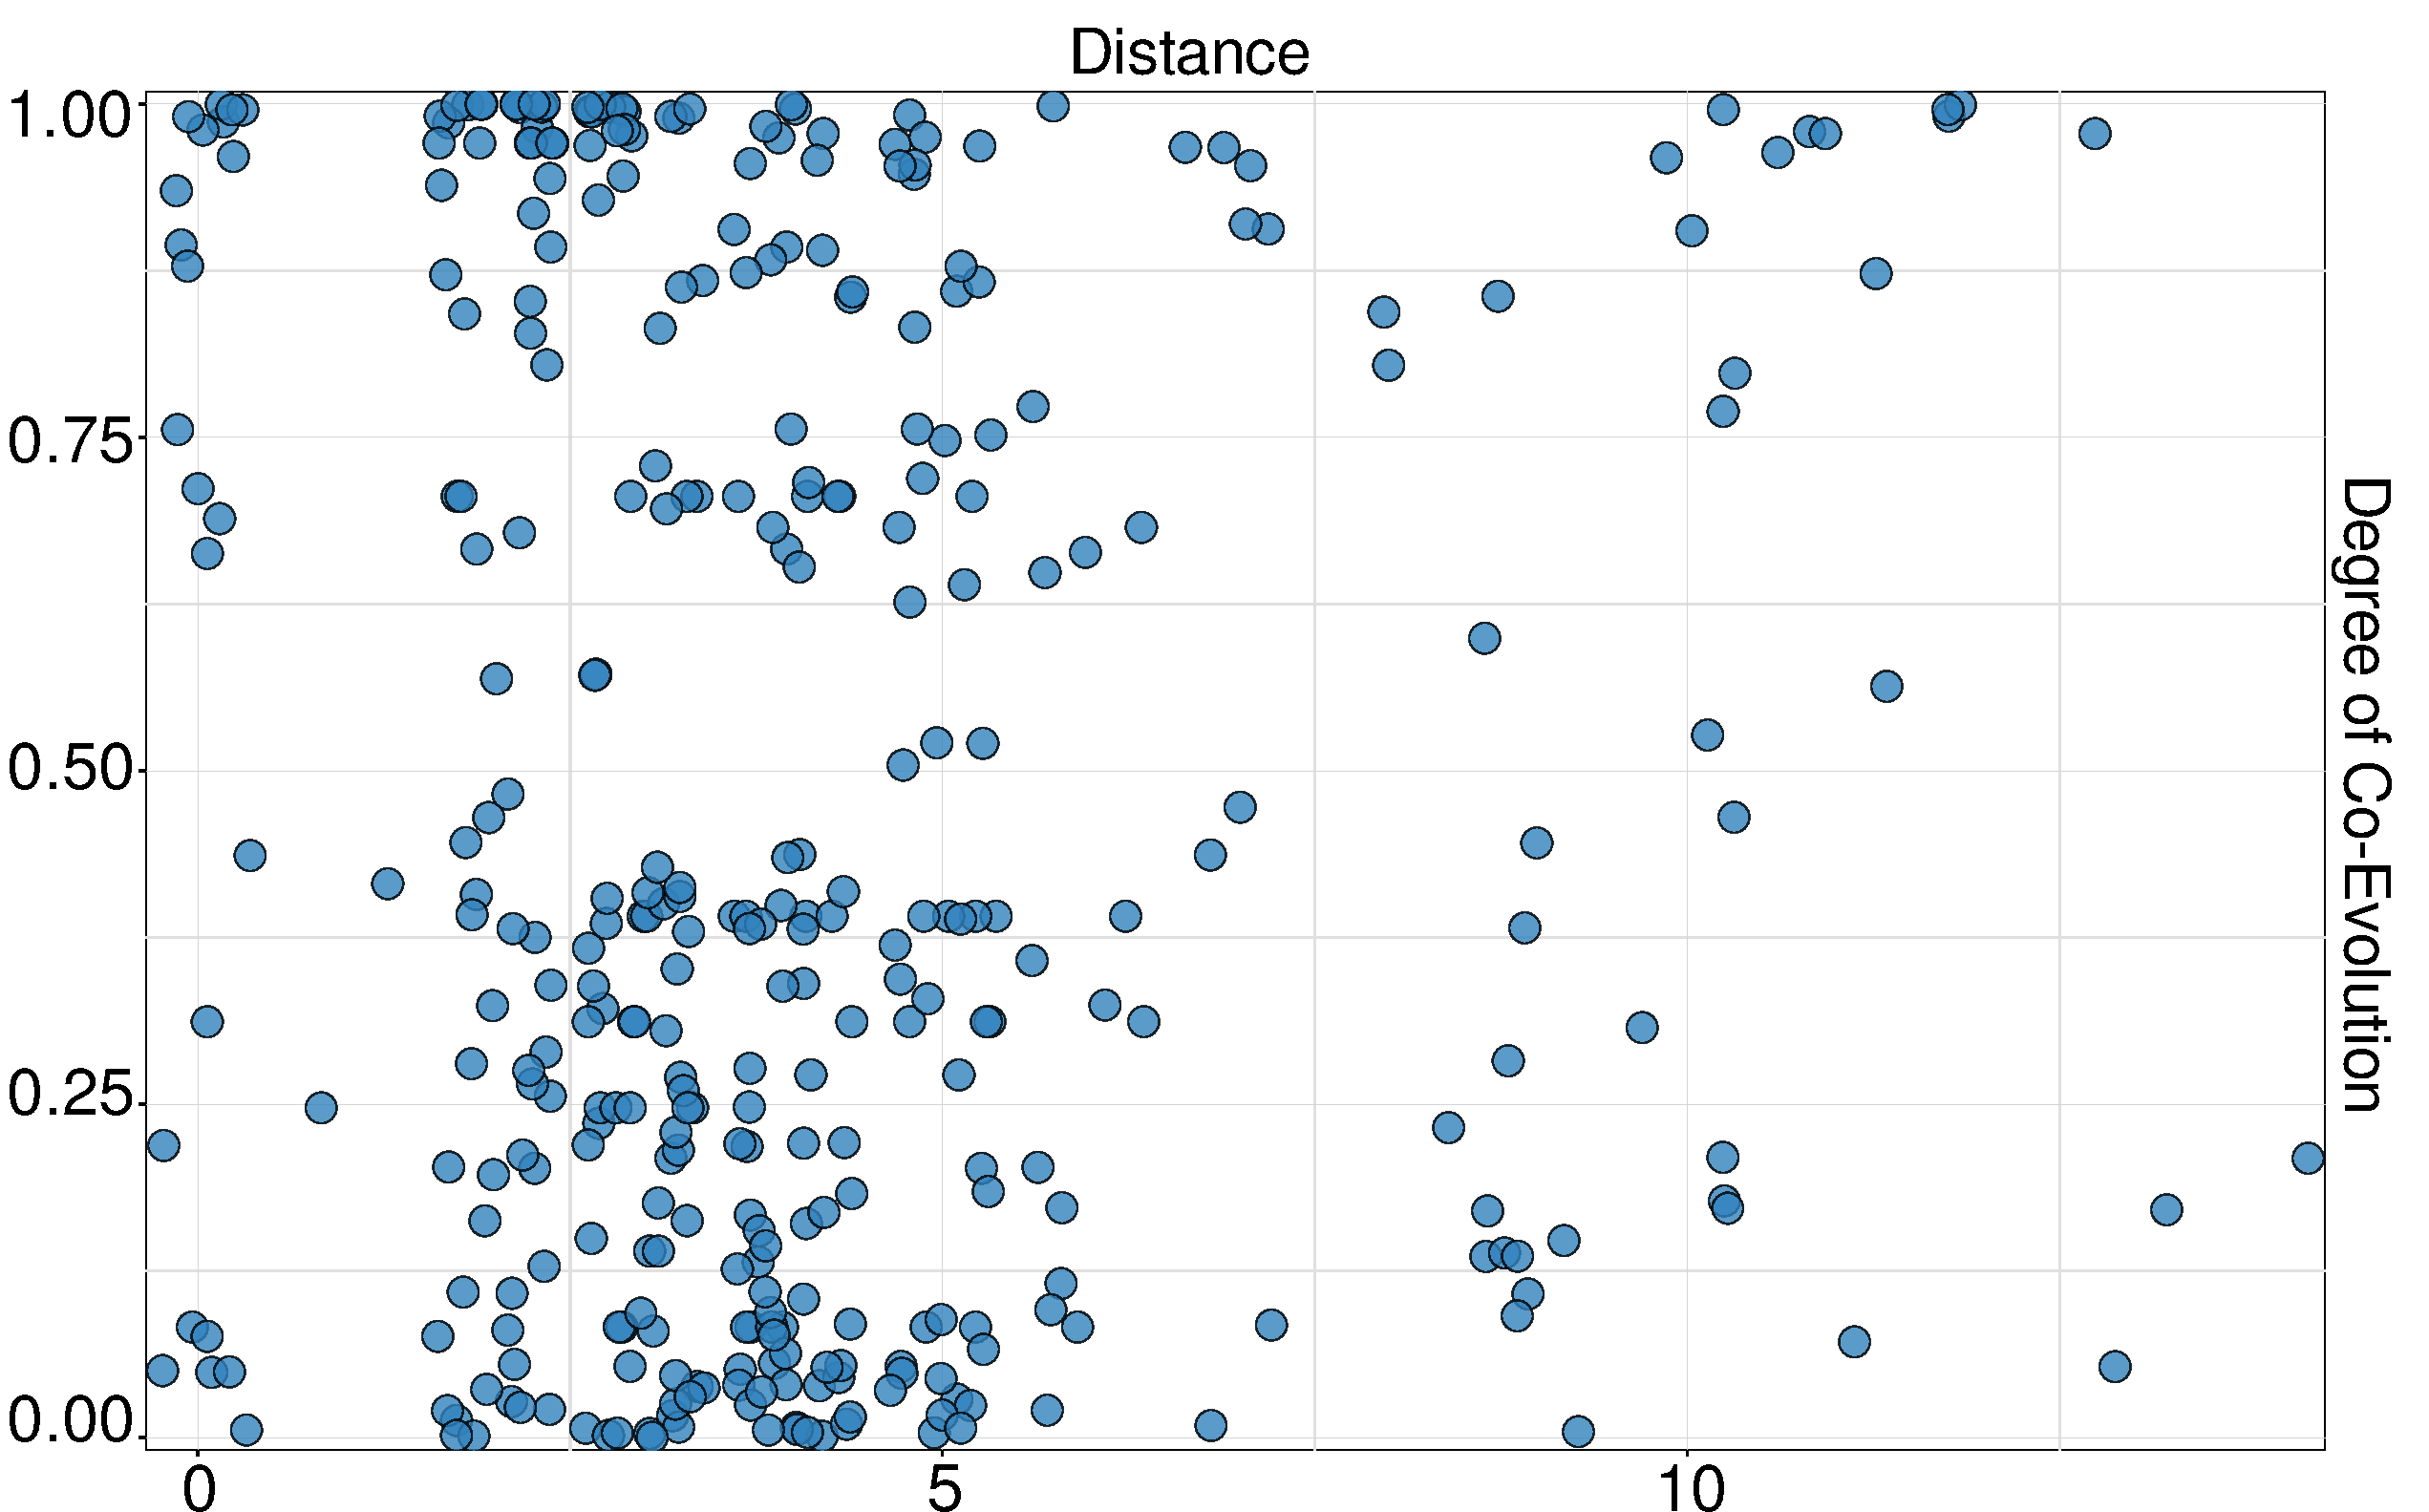
\includegraphics[width=.98\linewidth]{bpm2017/figures/Co-EvolutionVSDistance-OneColor.pdf}
		\caption{Distribution of pairs on real projects}
		\label{fig:pairs-on-space}
	\end{subfigure}
%	\vspace*{-.5cm}
	\caption{Characterization of the evaluated software projects}
\end{figure}
Next, we evaluate whether the work on files can be predicted. Zipf's law is typically used in corpus analysis and states that the \emph{frequency} of usage of any word is inversely proportional to its \emph{rank} in the frequency table. This approach has already been applied to software projects for understanding whether the assignment of developers to tasks in a software project could be predicted~\cite{Canfora2006}. Here, we focus on understanding whether the Zipf's law holds true also for work dependencies within a project. 

To this end, we selected one big and one small project from \Cref{table:evaluation-results-new}, namely \emph{Biglist} and \emph{Caret}. Biglist is a small project on a list of strings which are known to cause issues when used as user-input data. Caret is a big project consisting in the development of a sublime text editor for Chrome OS.
We collected how frequently were the artifacts worked on to generate a ranking. \Cref{fig:zipf-graph} depicts the corresponding charts and the fitted Zipf distribution. We notice that both projects present a similar distribution of values. This holds also for the other projects analyzed. In particular, Zipf's law is valid for the most frequently changed files. Afterwards, the distribution drops because of files not being worked anymore but still being part of the project.
%In pure software development projects, the tail can hint at some dead code and the need for maintenance.

\begin{figure}[t]
%	\centering
	\begin{subfigure}{.5\textwidth}
		\centering
		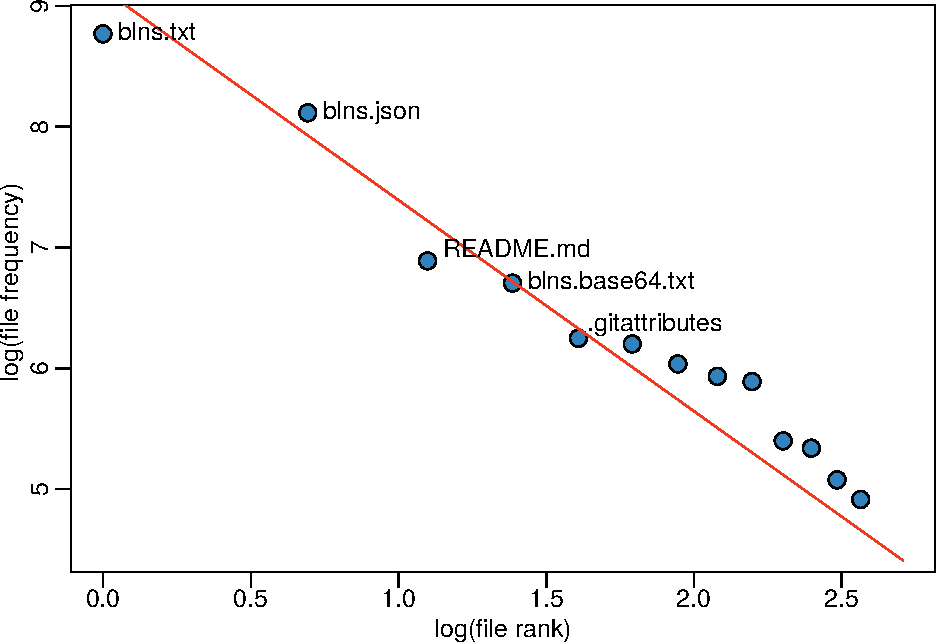
\includegraphics[width=\linewidth]{bpm2017/figures/biglist-new-crop}
		\caption{Biglist project}
		\label{fig:biglist}
	\end{subfigure}%
	\begin{subfigure}{.5\textwidth}
		\centering
		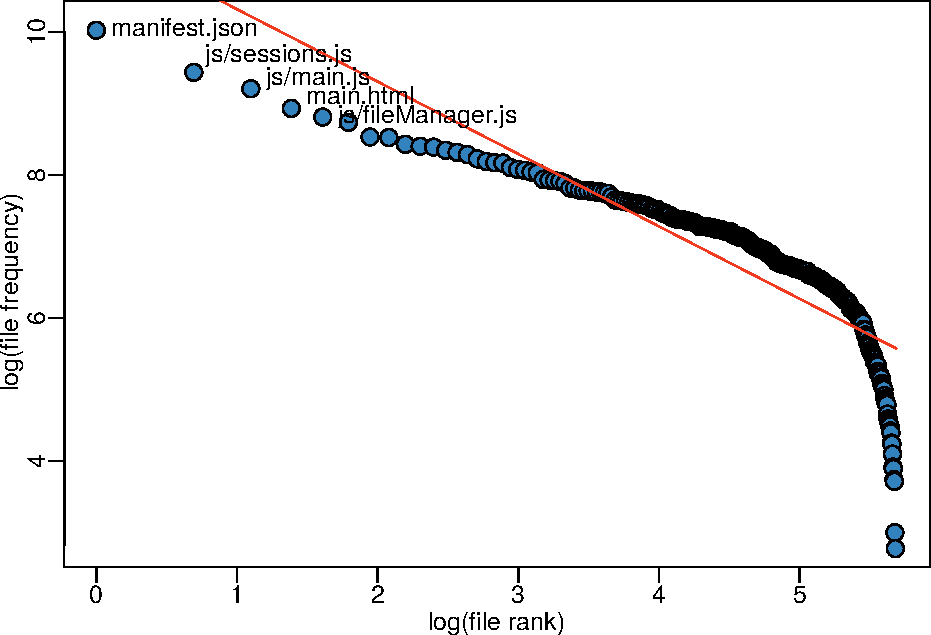
\includegraphics[width=\linewidth]{bpm2017/figures/caret-new-crop}
		\caption{Caret project}
		\label{fig:caret}
	\end{subfigure}
%	\vspace*{-.3cm}
	\caption{Zipf distribution of the worked files}
	\label{fig:zipf-graph}
\end{figure}
%\vspace*{-.2cm}